%% Full length research paper template
%% Created by Simon Hengchen and Nilo Pedrazzini for the Journal of Open Humanities Data (https://openhumanitiesdata.metajnl.com)

\documentclass{article}
\usepackage[english]{babel}
\usepackage[utf8]{inputenc}
\usepackage{johd}
\usepackage{fontspec}
\usepackage{csquotes}
\usepackage{longtable} %long tables
\usepackage{lscape} %mode paysage
\usepackage{tabularx}
\usepackage{tabularray}
\usepackage{graphicx}
\usepackage{float} %handle floats in metrics
\usepackage{subcaption} %handle subfigures
\newfontfamily{\junicodeFont}{JunicodeTwoBeta.ttf}
\newcommand{\juni}[1]{\textsf{\junicodeFont #1}}%
\usepackage{multirow}
\usepackage{color,soul}

\title{CREMMA Medii Aevi: Literary manuscript text recognition in Latin}

\author{%
    Thibault Clérice$^{a}$$^{*}$,
    Malamatenia Vlachou-Efstathiou $^{b}$,
    Alix Chagué $^{c}$  \\
    \small $^{a}$ Centre Jean Mabillon, École nationale des Chartes, PSL University, Paris, France \\
    \small $^{b}$ École nationale des Chartes, PSL University, Paris, France \\
    \small $^{c}$ INRIA, CNRS, Paris, France \\
    \small $^{*}$ Corresponding author: Thibault Clérice; \tt{thibault.clerice@chartes.psl.eu}
}


\date{} %leave blank

\begin{document}

\maketitle

\begin{abstract} 
\noindent %
This paper presents a novel segmentation and handwritten text recognition dataset for Medieval Latin, from the 11\textsuperscript{th} to the 16\textsuperscript{th} century. It connects with Medieval French datasets as well as earlier Latin datasets, by enforcing common guidelines, bringing 263,000 new characters and now totaling over a million characters for medieval manuscripts in both languages. We provide our own addition to Ariane Pinche's Old French guidelines to deal with specific Latin cases. We also offer an overview of how we addressed this dataset compilation through the use of pre-existing resources. With a higher abbreviation ratio and a better representation of abbreviating marks, we offer new models that outperform the Old French base model on Latin datasets, improving accuracy by 5\% on unknown Latin manuscripts. %
% A short (up to 250 words) summary of the main contributions of the paper and the context of the research. Full-length papers discuss and illustrate methods, challenges, and limitations in the creation, collection, management, access, processing, or analysis of data in humanities research, including standards and formats. These aspects must not necessarily be discussed with reference to a specific dataset (or collection thereof) but, if your paper focuses on particular datasets, we advise adding the dataset metadata under the section ‘Dataset description’. This template provides a general outline for full-length papers and authors can adapt the headings and include subheadings as they find appropriate. Please delete or replace the blue text with your own text in black. %
\end{abstract}

\noindent\keywords{Handwritten Text Recognition; Latin; manuscripts; Middle Ages; Layout Segmentation }\\

\noindent\authorroles{Thibault Clérice and Alix Chagué were responsible for the project administration. TC supervised and curated the data of the project. Malamatenia Vlachou-Efstathiou and TC produced the data, MV-E contributing more than half of the  transcription work. All contributed to the writing of this paper.} 

\section{Context and motivation}

\paragraph{Institutional and academic contexts}

Handwritten text recognition (HTR) and its upstream task layout segmentation (LS) have become two important topics in the context of Digital Humanities and digital approaches to cultural heritage collections in the GLAM\footnote{Gallery Library Archives Museums.} domain. Its growth over the past three to four years in digital projects can easily be linked to the emergence of user interfaces (UI) allowing for the annotation of ground truths (GTs, data that will be used for training), training new models (for the transcription and also, lately, for the segmentation) and for the automatic transcription of the users' own data. At first, only Transkribus \citep{kahle2017transkribus} provided such a service through the READ project without fees or infrastructure requirements.\footnote{\url{https://readcoop.eu/our-story/}} At the end of the 2020 European Union funding, Transkribus became a paid service which accelerated the interest growth of at least one alternative, namely eScriptorium \citep{kiessling2019escriptorium} at the EPHE-Scripta-PSL. Unlike the former, the latter is completely open-source, at the cost of not offering a centralized server.

In this context, the \textit{Consortium pour la Reconnaissance d’Écritures Manuscrites des Matériaux Anciens} (CREMMA) project was created to fund a regional server. Its aims are to support students' training and to provide local researchers with a free solution, in exchange for guaranteeing the release of data. The CREMMA funding consisted of a starting grant for the initial cost of the infrastructure (graphic cards, servers, routers, etc. for around 42,000€ VAT excluded) as well as an evaluation grant for providing base models for the community of CREMMA's users (around 8,000€). The latter was divided into two main languages: French and Latin, from the 9\textsuperscript{th} to the 21\textsuperscript{st} century. A postdoctoral position, CREMMAlab, provided the infrastructure with complementary time for building a dataset (CREMMA Medieval) and expertise around transcribing medieval manuscripts.

As the CREMMA project was being drafted, \cite{Chague_HTR-United_Ground_Truth} provided a solution for facilitating the FAIR principles (findability, accessibility, interoperability, reusability) in an HTR context and providing machine-actionable metadata for datasets. \textit{HTR-United}, both a catalog of open source HTR ground truth and a toolkit to strengthen the control of documentation and validity of HTR data, is born from this necessity, and offers, as of late October 2022, 56 datasets composed of 41.5 million characters, 725,862 lines in over 13 languages and 6 scripts. By designing \textit{HTR-United} we became aware of the stakes of spending our budget in the creation of new corpora and models. They are useful and can complement other existing projects.

\paragraph{HTR for Latin and Old French}


Handwriting in the middle ages can generally, and in a simplistic way, be divided into two big writing systems: cursive and calligraphy \cite[pp.~58 sqq.]{bischoff1985paleographie}. They reflect two complementary practices, namely cursive hands (\textit{écritures d'usage}) - which are more common to everyday documents such as accounting books, charters, letters, intellectual work - and book hands.\footnote{The distinctive functions gradually ceased to exist/converged as they were used interchangeably depending on the context.} While cursive represents a harder challenge due to the variability of handwriting styles, both families have the particularity to be potentially highly abbreviated, depending on the expected audience of the document: literary classics such as Cicero or Vergilius might be less abbreviated than pharmaceutical recipes, scholastic works, or accounting books of an abbey. This situation resulted in mainly two different kinds of \textit{HTR} ground truth dataset creation strategies: (1) datasets that would resolve abbreviations directly in the transcription (a practice found mostly used by historians, and quite common for cursive, at least in France) and (2) datasets that would keep a diplomatic approach to transcription.

%While resolving abbreviations produces specific difficulties for HTR engines, as it leads them to learn more about the language than they are originally intended for, diplomatic transcriptions entail their respective difficulties, specifically regarding the way in which transcribing specific letters should be handled. Diplomatic transcription can range from graphetic (for which all variations of the signs, be it letters or punctuation signs, are differentiated) to graphemic (preserving the sequence of signs but reducing them to a standardized representation in the alphabetical system) transcription. These two approaches present their own level of granularity, given that neither all variations of characters are available in the UTF8 standard nor do they exist in the private zone filled by projects such as the Medieval Unicode Font Initiative (MUFI) nor do all transcribers recognize the sometimes minor differences between different instances of the same character. For example, one project might be concerned specifically with differentiating only between \juni{ſ} (long s) and s, as it is one of the only character variations that were common at least until the end of the 19\textsuperscript{th} century, including in print.
 
Our dataset builds on the experience of Ariane Pinche and specifically her work on the CREMMA Medieval dataset, which treats different variations of Old French from the 13\textsuperscript{th} to the 15\textsuperscript{th} century, with a heavy focus on the first section of the period. It started as an adaptation of \cite{pinche_edition_nodate} into an OCR dataset and follows our common work regarding HTR and stylometric analysis \citep{10.1093/llc/fqab033}. During her postdoctoral work, Pinche co-organized a research seminar around the formalization of transcription guidelines for graphemic transcription of Old French \citep{pinche:hal-03697382}. It notably involved French and Swiss medievalists, including Stutzmann, who applied HTR to a large amount of data in the framework of the HIMANIS project \citep{bluche2017preparatory}, opting for the resolution of abbreviations in their data.

% Cite https://arxiv.org/pdf/2207.07726.pdf

Based on the work from Pinche, a few datasets emerged around the École nationale des Chartes and the CREMMA project. Notably, the GalliCorpora corpora \citep{gallicorpora15} and the course project DecameronFR \citep{DecameronFR} provided two additions for Old French and Middle French data, centered around the end of the middle ages. On the opposite, the Caroline Minuscule project \citep{hawk2018modelling} was realigned with original images and adapted to our guidelines and datasets format (ALTO XML) for eScriptorium, as it provided some foundations for recognizing the Caroline script specific to the first centuries of the early middle age. On top of this project, \cite{vlachou-efstathiou2022voss} provided a dataset based on the transcriptions of two Latin manuscripts from the 9\textsuperscript{th} century. At the start of the present dataset production, there was a lack of data for the second half of the middle age (1100-1500) which we focused on for our dataset (see Table \ref{tab:datasets}).

\begin{table}[]
    \centering
    \resizebox{\linewidth}{!}{%
    \begin{tabular}{lllrrr}
         \hline
         Authors & Dataset & Project & Characters & Period & Language\\ \hline
         \cite{caroline} & Caroline Minuscule & Rescribe & 17,000 & 800-1200 & Latin\\
         \cite{eutyches} & Eutyches & - & 87,000 & 850-900  & Latin \\ 
         \cite{cremmaMedieval} & CREMMA Medieval & CREMMA(lab) & \textbf{593,000} & 1100-1499  & French\\
         \textit{-} & \textbf{CREMMA Medii Aevi} & CREMMA & 263,000 & 1100-1600  & Latin \\
         \cite{DecameronFR} & DecameronFR & - & 20,000 & 1430-1455 & French \\
         \cite{gallicorpora15} & Manuscrits du 15e siècle & GalliCorpora & 169,000 & 1400-1500 & French \\ \hline
         \textbf{Total} & & & 1,149,000 & &  \\ \hline
    \end{tabular}}
    \caption{Datasets following the Pinche Guidelines, or adapted through Choco-Mufin. Characters' counts are rounded to the closest thousands.}
    \label{tab:datasets}
\end{table}

\section{Dataset description}

\paragraph{Object name} Typically the name of the file or file set in the repository.
\paragraph{Format names and versions} XML (ALTO), JPEG
\paragraph{Creation dates} 2022-01-01 / 2022-09-22
\paragraph{Dataset creators} Thibault Clérice (Organization, Curation, Transcription, Design), Malamatenia Vlachou-Efstathiou (Curation, Transcription, Design), Alix Chagué (Organization)
\paragraph{Language} Latin
\paragraph{License} CC0
\paragraph{Repository name} Zenodo
\paragraph{Publication date} 2022-09-XX

\section{Method}

\subsection{General aspects of the corpus}

\paragraph{Corpus construction theory}

Borrowing the terminology from the linguistic domain \citep{bauer2000corpus}, where data construction methods have long been examined, evaluated, and reconsidered, we shall examine the following methodological aspects. Contrary to the notion of \enquote{sampling} which is by definition a random selection procedure, \enquote{corpus construction} implies a systematic selection of materials that obey a specific rationale, where its efficiency depends on the research question. \enquote{Representative sampling} is where these two approaches converge.
Sampling secures efficiency in research by providing a rationale for studying only parts of a population without losing information. Its key feature is \enquote{representativeness} of the system in question. The larger the range of population representation the smaller the error. Sampling criteria and focal variables correlate. Language corpora and specifically those oriented towards formal criteria (handwriting) rather than content (dialects etc.) are easier to deal with than population or natural language corpora. In HTR for medieval manuscripts, \enquote{representativeness} was approached in terms of the medieval handwritten Latin language's characteristics -- as a system comprised of abbreviations, ligatures, and punctuation signs alongside graphemes. Different genres, scripts, and their degrees of formality served as instances of this system.\footnote{More specialized studies concerning quantitative approaches in codicology and paleography like \citep{maniaci1993che} other than theoretical factors, stress practical factors such as availability, medium, diversity, and internal homogeneity}  
%Indeed, the choice of individuals to be examined is oriented, from the outset, according to the hypotheses from which the investigation takes its starting point and which are expressed, indirectly, in the identification of a coherent set of parameters to be observed.
%In essence, contrary to what one would naturally tend to assume, scientific performance depends not so much on the "intrinsic richness" of individual variables, but rather on the number of relationships that can be established between one and another of them.

\paragraph{Document sampling strategy}

From the three registers making up the construction of a qualitative corpus according to \cite{bauer2000corpus}, namely channel, domain, and function, only the first parameter is constant in our case: the sample represents exclusively the written Latin language, while giving room to texts of multiple functions addressed to different audiences belonging to various genres (while not aiming at exhaustiveness at this stage). The corpus construction can be regarded as a cyclical process: it has not been entirely determined \textit{a priori} but rather evolved, bearing in mind the logic of complementarity regarding the already existing datasets. Statistical features, such as abbreviation rate or use of specific characters, can only be estimated from afar and only the analysis of the transcriptions could provide feedback for selecting new documents to fill the gap or strengthen some features. Different genres and scripts were implemented to compensate for what was thought to be missing from the corpus in order to render it as \enquote{representative} as possible. HTR engines are language agnostic, but the same cannot be told for the resulting models, which means that it depends on the representativeness of the sample to determine whether a model will work on ``similar'' documents. The selection of variables can only take place within the framework of a dialectical process in which knowledge of the object and the historical substratum, acquired preliminarily, feeds and controls the prediction.

%We respected in any case the criteria of relevance (to the research topic and the end goal) and homogeneity (in terms of non-combining different media) but not that of synchronicity ("The normal cycle of change will define the time interval within which a corpus of relevant and homogeneous materials should be selected") since no particular natural cycle was considered, instead, the logic was that of complementary to what exists already (that way both Gothic and humanistic scripts were considered).

Three distinctive selection processes have been applied in our case:
\begin{enumerate}
    \item The first set of documents was selected purely on their linguistic feature, their readability, and their availability as both digitized manuscripts and editions which could be found either online or in local libraries. It led to the inclusion of mostly classical texts such as Seneca's \textit{Medea}, and the \textit{Priapea}. The script did not dictate this selection step.
    \item In a logic of complementarity, the second part of the corpus was dictated, inversely by content. More specifically, given the relative absence of ligatures and abbreviations in classical texts, an important feature of medieval handwritten practices, documents that would display a higher degree of abbreviations were chosen. This led to a genre selection process, specifically for medical and scholastic data. At the same time, and always seeking not to repeat already existing features for the sake of saturation, script diversity was added to the consideration and came naturally as a sort of by-product. 
    \item Finally, as we wanted to test Kraken models, we sought a transcription project that would provide us with data that would help us evaluate our own. This led to the inclusion of \cite{eichenberger_nicole_2021_5582483} dataset, produced in the context of a transcribathon in Berlin, in the CREMMA Medii Aevi corpus: it contains a new genre of documents for the corpus (Book of Hours, Psalms, etc.).
\end{enumerate}

% Pilot empirical investigation (we start from something, observe what lacks, what could be added, what would be useful) leads to a more concrete corpus design, and recompiling a portion of the corpus paves the way to a more concrete strategy. In other words, (1) select preliminary, (2) analyze, and (3) extend the corpus until saturation. This way a cyclical process occurs, which gives due recognition to two rules of corpus construction according to \cite{bauer2000corpus}: (1) external variation precedes awareness of internal variation, and so corpus construction has to start from different contexts, (2) the aim is to maximize internal variety through the extension of the functions, registers, or genres that are being considered.


\paragraph{Quantitative aspects of the corpus}

Size depends largely on the subjective criteria and resources of each project and little can be said as a general rule: one needs to consider the limitations that stem from the effort put into producing the corpus, the budget available, the number of representations one wants to characterize, and some minimal and maximal requirements (in our case the quota for the production of an efficient HTR model).

Building a turn-key HTR model applicable to as large a range of unseen manuscripts as possible is undoubtedly the end goal (cf. the work on CREMMA Medieval and CREMMA Lab mentioned above) With the production of ground truth being expensive but with increasingly more open-access models available to the public, the challenge is finding the right combination of GTs (either to create a model from scratch or to fine-tune an existing one) that yield the best results. This is where considerations of size and variety enter the discussion and affect directly the quantitative corpus construction strategy.

More specifically, while conducting an experiment on Caroline Minuscule OCR models, \cite{hawk2018modelling} conclude that \enquote{relative preponderance}\footnote{the proportionally higher or lower representation of a manuscript or subgroup of manuscripts in the training pool and the subsequent effect on the accuracy of the respective test manuscript or subgroup.} in small training pools was a considerably more important factor than that of size, which inversely impacts the accuracy of the models resulting from larger training pools. A careful conclusion would have it that a specific combination of manuscripts can yield exceptional results, even though the reasons behind such results or the criteria for the respective manuscripts to be combined are not entirely clear yet. This means that quantity-wise we sought to find a balance between diversity and size of the GT, always making sure that the ground truth yields an efficient model for individual manuscripts on the training set. Training and fine-tuning experiments conducted by Pinche showed that a specialized model per script isn’t always necessary, but the variety of the training set increases its robustness. Therefore, the size of each GT belonging to the train set  was limited to 5 pages per script variation (depending on the density of the layout)\footnote{Aside from 3 documents coming from the Berlin Transcribathon, that were utilized rather as evaluating tools at the end of the project.}, examining whether this balance can contribute to the production of a generic models.\footnote{On GT size for OCR experiments see: \cite{strobel2020much}.}

\paragraph{Segmentation vocabulary: SegmOnto}

With the emergence of efficient layout analyzers and easy-to-use interfaces, the need for efficient segmentation models increases, as does the need for large amounts of data, based on the aggregation of heterogeneous documents. For this, researchers need to agree on a limited common vocabulary and share common practices to facilitate the interoperability of their ground truth.

Alongside text recognition, eScriptorium allows for layout annotation using ontologies and controlled vocabularies. A controlled vocabulary is a lexicon whose purpose is to enable the organization of knowledge to optimize information retrieval and requires the use of terms predefined by the vocabulary designer. In order to identify the different areas of the document and the type of lines present on the page as well as to characterize them from a codicological point of view, we decided to implement the controlled vocabulary \textit{SegmOnto} \citep{gabay2021segmonto}. \textit{SegmOnto} was born out of the need for a limited common ontology based on existing standards, for the description and analysis of document layout, ranging from content categorization to text recognition, mainly addressing the case of manuscripts and early printed books. 

\textit{SegmOnto} has already been implemented in several projects led by Pinche and connected to the CREMMALab project such as \cite{gallicorpora15}, resulting in segmentation models mainly for late medieval manuscripts and early prints.\footnote{More information and case studies can be found here: \url{https://segmonto.github.io/}.} As per the CREMMA Medii Aevi dataset, the documents present two kinds of layout: multi-columns and singular columns, for which lines are most often long, except for the Psalms and Book of Hours. SegmOnto offers multiple levels of description, of which only one is completely standardized (the first level), as the second is intended for custom refinement and the third for local and document-based differentiation. For the purposes of the project, only the first level of \textit{SegmOnto} has been utilized, notably, the \texttt{MainZone} and occasionally the \texttt{MargintextZone} for \texttt{marginalia}, and the \texttt{DefaultLine} tag for the characterization of the lines. 

\paragraph{Pinche's Guidelines} \label{pincheguidelines}

\cite{pinche:hal-03697382} stressed the fact that due to the need for scientific projects to acquire textual data in mass either to undertake editions of long texts or to constitute large corpora to be interrogated, the use of HTR is becoming necessary to process such a mass of data. The guidelines are the result of the need to establish principles common to projects dealing with the transcription of manuscripts in order to:
\begin{itemize}
    \item accompany the creation of training seeking to optimize the machine learning of HTR models;
    \item build shareable and reusable ground truth data sets;
    \item produce robust generic models, reusable in ``out-of-domain'' manuscripts with or without customization, useful to the scientific community;
    \item minimize the collective cost, including that of training people;
    \item ensure the durability and reuse of the data produced. 
\end{itemize}

A graphemic transcription has been privileged instead of a graphetic one that reproduces the manuscript as truthfully as possible.\footnote{See \cite{camps2021creation}. On this particular topic, we share an opposite view with \cite{gueville:halshs-03725166}. However, while graphemic transcription can not be used for automated graphetic transcription, graphetic transcriptions can be turned easily into graphemic ones, at the cost of establishing a \enquote{translation} table for each character.} Pushing the imitation too far through a graphetic approach induces a risk of making the transcription harder to complete (as it requires technical skills to recognize differentiated shapes of characters), harder to make uniform (specifically as more annotators are to participate in a dataset) and potentially unusable for HTR (as it might introduce more characters and ultimately noise for HTR engine to learn). A graphemic transcription preserves the sequence of letters and reduces each form to its meaning and each letter \enquote{shape} to a standardized representation in an alphabetical system. %Instead of looking for over-refining the choice of Unicode signs in order to cover every variation of a grapheme, in order to avoid the multiplication of signs one representation corresponds rather to various instances.
Therefore, in cases where functional signs have more than one graphetic manifestation but essentially the same function, they could be represented by the same signv: for example, for every manifestation of the paragraph sign, we opt for the pilcrow sign \enquote{\juni{\symbol{"00B6}}} (U+00b6) on every occasion, instead of several variations such as the \textit{Paragraphus} sign \enquote{\juni{\symbol{"F1E1}}} (U+F1E1), for the sake of homogeneity (\textit{cf.} Table \ref{tab:all_punct}).\footnote{While most of the special characters exist as such in MUFI a conscious effort has been made to avoid as much as possible the private domain of MUFI, so the data can be as reusable and flexible as possible.}

%comment: do you have any example where resolving of abbreviations was useful ? - In projects with editions as the main goal (maybe mention the article of JBC and Chahan and Marguerite on resolving abbreviations?)
On the topic of abbreviations, resolving them produces specific difficulties for HTR engines, as it leads them to learn more about the language than they are originally intended for.\footnote{Most HTR engines learn directly from transcriptions: it means that it does not \enquote{know} when it's resolving abbreviation. Transcriptions produced by these models are thus not showing where an abbreviation was resolved, making it difficult to distinguish HTR errors from transcription resolution errors. The stakes do not specifically concern the scores, which seem to be close to each other \citep{camps2021handling}, but the long-term use of ground truth data and silver data in a sustainable way.} In our dataset, abbreviations are not resolved as this constitutes rather an interpretative act linked to the specificity of each document and it is not the same as a textual prediction and it could prove to be detrimental to the extension of an HTR model in the long term. However, as noted regarding the graphetic and graphemic distinction, diplomatic transcriptions entail their respective difficulties, specifically regarding the way in which transcribing specific letters should be handled. Graphetic and graphemic approaches present their own level of granularity, given that neither all variations of characters are available in the UTF8 standard nor do they exist in the private zone where projects such as the Medieval Unicode Font Initiative (MUFI) abound, nor do all transcribers recognize the sometimes minor differences between different instances of the same character. %Thus, in order to train HTR models, graphical transcriptions that preserve the original abbreviations and punctuation seems to be the most suitable. While abbreviations are preserved, ligatures composed of different characters are reduced to their components.
By setting up a list of allowed characters and a list of common and rare cases (such as Table \ref{tab:all_punct} and \ref{tab:all_abbr}), while not requiring much in terms of interpretation of the text, we allow for a simpler transcription step through reducing the characters diversity, ultimately satisfying both the human transcriber and the HTR engine in terms of learning curves.
 
In order to ensure the rigorous application of these guidelines and the homogeneity of the data produced, quality control softwares are introduced to the pipeline. Each corpus was passed through ChocoMufin \citep{Clerice_Choco-Mufin_a_tool_2021}, using project-provided character translation tables. This software, alongside these tables, allows for each dataset to be both controlled at the character level and adapted to guideline specifications and modifications. It also allows for project-specific transcription guidelines to be translated to a more common one such as CREMMALab’s one \citep{pinche2022cremmalab}.\footnote{In order to read the translation  table (generally named table.csv in ChocoMufin using repositories), MUFI compatible fonts are recommended, such as Junicode: \url{https://github.com/psb1558/Junicode-font}.} This process has been largely used in the first months of the CREMMA Medieval project, as the guidelines were still being drafted: it allowed Pinche to produce or align datasets first, and harmonize later, as long as the harmonization was from an upper level of details (closer to graphetic) to a lower level (closer to graphemic).

\subsection{Transcription Guidelines for the CREMMA Medii Aevi}

The section that follows aims to guide the reader through the transcription norms followed for the \textit{Medii Aevi} dataset, illustrating the process and the more common and complex cases, especially where new characters have been introduced compared to the \textit{CREMMA Medieval} dataset.

As a member of the CREMMA initiative, the project adheres to the general principles laid out by Pincghe \cite[Tables pp.~4-15]{pinche:hal-03697382} concerning the base cases (punctuation, word separation, functional signs, superscript letters, abbreviations, ligatures, and roman numerals). In cases of incoherence on a character level, mostly when there was a misunderstanding between transcribers, \enquote{incorrect} characters are handled automatically by ChocoMufin. Using the project-provided character conversion table, ChocoMufin controls the transcription and corrects any anticipated error by transforming automatically the character so it conforms to the pre-defined guidelines. This example stresses the fact that data should be used in their post-ChocoMufin control or \textit{ChocoMufined} state (manually or in the releases). However, where the guidelines were not directly addressing the situation (new characters, new types of abbreviations), we positioned ourselves and interpreted the guidelines in light of the situation: each decision was discussed with the original guidelines' author.\footnote{This include discussion with other projects, such as \cite{textasimages}, which led to the inclusion of the striken-through D (see Table \ref{tab:all_abbr}).}

% in terms of specific principles, what is important for every new project is to position itself against the existing ones and to find solutions for new special characters that are not already handled by previous guidelines, always bearing a graphemic approach in mind.

%Maybe unnecessary, or at the end?
In general, the main differences that we isolated between the CREMMA Medieval and Medii Aevi datasets, stemming from the language as well as the genre's own characteristics, are:
\begin{enumerate}
    \item the dataset bears no accentuated vowels like in the Old French texts (a rare event though for the corpus);\footnote{This is different from \texttt{i} pointing, which is not taken into account by either corpus.}
    \item no normalization of \texttt{u} and \texttt{v} was provided, nor of \texttt{i} and \texttt{j};\footnote{They are however undistinguished ultimately by the newer version of guidelines.}
    \item two variations of con (antisigma) and 9-shaped are found;
    \item a higher diversity of abbreviating character usage and signification;
    \item Arabic numerals alongside roman, mostly in scholastic and medical treatises.
\end{enumerate}

\paragraph{Reference marks, functional signs, and punctuation}

In general, complex medieval punctuation has been simplified as much as possible, with single sign punctuation being reduced to \enquote{\texttt{.}} and commas will be rendered as \enquote{\texttt{,}}. Double sign punctuation (mainly \textit{punctus elevatus} and \textit{punctus interrogativus}) are consistently reduced to \enquote{\texttt{:}}. The hyphenation for words that continue to the next line has been marked with a unique \enquote{\symbol{"002D}} (U+002D) sign, following \ref{pincheguidelines}. Table \ref{tab:all_punct} gives a representative example.

\begin{table}[H]
    \centering
    \resizebox{\linewidth}{!}{%}
    {\junicodeFont%
    \begin{tabular}{c|c|c|c|c}
        \hline
        Type & Transcription & Unicode & Description or resolution & Examples \\ \hline
        \multirow{2}{*}{Punctuation} & \multirow{2}{*}{¶} & \multirow{2}{*}{U+00B6} & \multirow{2}{*}{Content change} & 
            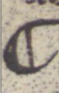
\includegraphics[height=1.5cm]{datapaper/images/examples/pilcrow/pilcrow_CML13027.png}
            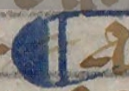
\includegraphics[height=1.5cm]{datapaper/images/examples/pilcrow/pilcrow_Maz915.png}
            
\includegraphics[height=1.5cm]{datapaper/images/examples/pilcrow/pilcrow_faded_CML13027.png}
            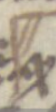
\includegraphics[height=1.5cm]{datapaper/images/examples/pilcrow/pilcrow_gamma_CML13027.png}
            \\
        & & & &
            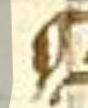
\includegraphics[height=1.5cm]{datapaper/images/examples/pilcrow/pilcrow_Montpelier.H 318.png}
            
\includegraphics[height=1.5cm]{datapaper/images/examples/pilcrow/pilcrow_red_CML13027.png}
            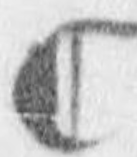
\includegraphics[height=1.5cm]{datapaper/images/examples/pilcrow/pilcrow_Latin6395.png}
            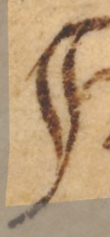
\includegraphics[height=1.5cm]{datapaper/images/examples/pilcrow/pilcrow_Laurentianus39.34.png}
        \\
        Punctuation & \symbol{"002D} & U+002D & Hyphenation & 
        \raisebox{-.5\height}{
            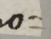
\includegraphics[height=1.5cm]{datapaper/images/examples/hyphen/hyphen_CCCC165.png}
            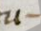
\includegraphics[height=1.5cm]{datapaper/images/examples/hyphen/hyphen_Plut 53.08.png}
            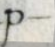
\includegraphics[height=1.5cm]{datapaper/images/examples/hyphen/hyphen_Plut.53.09.png}
        }
        \\
    Punctuation & \symbol{"2215} & U+2215 & Diastole & 
        \raisebox{-.5\height}{
            
\includegraphics[height=1.5cm]{datapaper/images/examples/diastole/BAV_pallat_373.png}
            
\includegraphics[height=1.5cm]{datapaper/images/examples/diastole/BIS193.png}
        }
        
        \\
        Reference mark & \symbol{"2038} & U+2038 & Omission sign 'caret'(reintroduction of content) & 
        \raisebox{-.5\height}{
            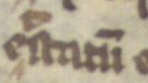
\includegraphics[height=1.5cm]{datapaper/images/examples/additions/addition_CML13027.png}
            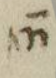
\includegraphics[height=1.5cm]{datapaper/images/examples/additions/addition_Sorbonne193.png}
            
\includegraphics[height=1.5cm]{datapaper/images/examples/additions/addition_VatLat373.png}
        }
        \\
                Punctuation & \symbol{"003A} & U+003A & Punctus elevatus & 
        \raisebox{-.5\height}{
            
\includegraphics[height=1.5cm]{datapaper/images/examples/punctuation/punctus_elevattus_MsWettF 15.png}
            
\includegraphics[height=1.5cm]{datapaper/images/examples/punctuation/punctus_elevatus_CML13027.png}
            
\includegraphics[height=1.5cm]{datapaper/images/examples/punctuation/punctus_elevatus_egerton821.png}
            
\includegraphics[height=1.5cm]{datapaper/images/examples/punctuation/punctus_elevatus_Latin 16195.png}
            
\includegraphics[height=1.5cm]{datapaper/images/examples/punctuation/punctus_elevatus_Latin6395.png}
            
\includegraphics[height=1.5cm]{datapaper/images/examples/punctuation/punctus_elevatus_Montpelier.H 318.png}
            
\includegraphics[height=1.5cm]{datapaper/images/examples/punctuation/punctus_elevatus_Phil10a135.png}
            
\includegraphics[height=1.5cm]{datapaper/images/examples/punctuation/punctus_elevatus_Plut 53.08.png}
        }
        \\
        Punctuation & \symbol{"003A} & U+003A & Punctus interrogativus & 
        \raisebox{-.5\height}{
            
\includegraphics[height=1.5cm]{datapaper/images/examples/punctuation/punctus_interrogativus_CCCC165n.png}
            
\includegraphics[height=1.5cm]{datapaper/images/examples/punctuation/punctus_interrogativus_Laurentianus39.34.png}
            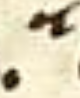
\includegraphics[height=1.5cm]{datapaper/images/examples/punctuation/punctus_interrogativus_Montpelier.H 318.png}
            }
            \\ \hline
    \end{tabular}
    }}
    \caption{Punctuation, functional signs and hyphenation.}
    \label{tab:all_punct}
\end{table}


 % For punctus elevatus and interrogativus \caption{In the following order, folder containing these samples: MsWettF 15, CML13027, Egerton821, Latin16195, Latin6395, Montpelier.H 318, Phil10a135, Laurentianus 53.08, CCCC165n, Laurentianus 39.34, Montpelier.H 318.}



\paragraph{Contractions, Abbreviations, and Ligatures}

\cite{cappelli1899dizionario} categorized abbreviations into six categories: truncation, contraction,  abbreviation marks significant in themselves, abbreviation marks significant in context, superscript letters, and conventional signs. As \cite{plutaabbreviations2020} stresses, the six aforementioned categories are not mutually exclusive, but the functional grouping is helpful.  

\textbf{Contractions}: A word is abbreviated by contraction when one or more of the middle letters are missing. Such an omission is indicated by one of the general signs of abbreviation, present in both corpora, always following \cite{pinche:hal-03697382}. Thus, macrons and generally horizontal lines diacritics over the letter such as tildes are represented by horizontal tildes, any zigzag similarly shaped forms are simplified into superscript vertical tildes. In our corpus, in cases where a macron is extended to more than one letter due to the cursivity of the script, this trait has been reproduced in the transcription, as well as in the case of stacked diacritics, usually in later medieval manuscripts (\textit{cf.} Table \ref{tab:all_lig}).

\textbf{Abbreviation marks significant in themselves}: \enquote{Standard} Abbreviations signs have been preserved as such, like \textit{pr(a)e} -\juni{p\symbol{"0303}} (p + combining tilde, p + U+0303),  \textit{pro} -\juni{ꝓ} (U+A753), \textit{hoc} - \juni{ħ} (U+0127), \juni{\symbol{"1E9C}} (s with diagonal stroke, U+1E9C) for \textit{secundum} or \textit{ser-}, \juni{ꝯ} for 9 shaped \textit{con}/\textit{cum} (U+A76F), Tironian sign \juni{\symbol{"A770}} for the desinence \textit{-us} (U+A770), \juni{\symbol{"2007}\symbol{"1DD1}} for \textit{(t)ur} (U+1DD1),  and \juni{\symbol{"A758}}/ \juni{\symbol{"A759}} for \textit{quod}. Absent from the CREMMA Medieval but present in Medii Aevi (U+A758/U+A759), the truncated ending \textit{-is} is transcribed using the character \juni{\symbol{"A76D}} ("U+A76D). 
The \enquote{inverted c} variation of the preposition con/cum is a good example for the difference of approach between the graphetic and graphematic approach: while using the \textit{antistigma} (\juni{\symbol{"2184}}) might look interesting for a graphetic approach, it simply is a variation of the original \juni{ꝯ} which is used. For \textit{-rum}, in a graphemic transcription, the symbol \juni{\symbol{"A775}} is used rather than the specific rotunda -rum \juni{\symbol{"A75D}} (U+A75D) of the MUFI.\footnote{The same two-shaped mark on the baseline, combined with a downward stroke, may stand as well for ``-ris'' as in ``Aristoteles'', though it is more often used at the end for ``rum''.}

\textbf{Abbreviation marks significant in context} : The abbreviation for the enclitic \textit{-que} or simply -\textit{-bus} or vertical \textit{-m} in later manuscripts, has been reduced to the semicolon \juni{\symbol{"F1AC}} sign (U+F1AC), in order to avoid the ligature specific \juni{\symbol{"E8BF}} (U+E8BF) character belonging to the private domain of MUFI and in order to avoid confusion with the regular semicolon.

\textbf{Conventional signs}:  a category that includes all signs that stand for a frequently used word or phrase, and they are almost always isolated (\textit{cf.} \cite{plutaabbreviations2020}). 
First, a rather frequent one, the abbreviation sign for \textit{esse} is represented by the mathematical operation Almost equal \juni{≈} (U+2248) always abiding by the MUFI recommendations. In the same vein, the Division sign \juni{÷} is used ubiquitously for the abbreviation sign of \textit{est/id est}. Tironian \textit{et} (U+204A, all variations of it, \textit{cf.} below) is transcribed by \juni{⁊}. \textit{Etiam} can also be found abbreviated by a combination of the Tironian \textit{et} and the macron symbol, for which a horizontal tilde is used (see Table \ref{tab:all_lig}.).% As a compliment to this category, but specific to our dataset serves the \ref{special_chars} subsection.

\begin{table}[H]
    \centering
    \resizebox{\linewidth}{!}{%}
    {\junicodeFont%
    \begin{tabular}{c|c|c|c}
         Character(s) & Unicode & Resolution & Examples \\ \hline
         ⁊ & U+204A & Et & 
             \raisebox{-.5\height}{% This provides centering for text on the left by adjusting the baseline of the pictures
             
\includegraphics[height=1.5cm]{datapaper/images/examples/torinian_et/et_tironien_CLM13027.png}
             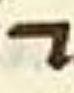
\includegraphics[height=1.5cm]{datapaper/images/examples/torinian_et/et_tironien_Montpelier.H 318.png}
             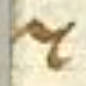
\includegraphics[height=1.5cm]{datapaper/images/examples/torinian_et/et_tironien_2_Montpelier.H 318.png}
             
\includegraphics[height=1.5cm]{datapaper/images/examples/torinian_et/et_tironien_Latin 16195.png}
             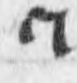
\includegraphics[height=1.5cm]{datapaper/images/examples/torinian_et/et_tironien_Latin6395.png}
             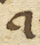
\includegraphics[height=1.5cm]{datapaper/images/examples/torinian_et/et_tironien_Phil10a135.png}
             
\includegraphics[height=1.5cm]{datapaper/images/examples/torinian_et/et_tironien_VatLat373.png}} \\
          ⁊+◌\symbol{"0303} & U+204A + U+0303 & Etiam & 
            \raisebox{-.5\height}{%
            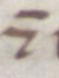
\includegraphics[height=1.5cm]{datapaper/images/examples/etiam/etiam_CML13027.png}
            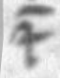
\includegraphics[height=1.5cm]{datapaper/images/examples/etiam/etiam_Latin 16195.png}
            
\includegraphics[height=1.5cm]{datapaper/images/examples/etiam/etiam_MsWettF 15.png}} \\
        \symbol{"A76D} & U+A76D & -is &
            \raisebox{-.5\height}{%
            
\includegraphics[height=1.5cm]{datapaper/images/examples/is/is_Sorbonne193.png}
            
\includegraphics[height=1.5cm]{datapaper/images/examples/is/is_VatLat373.png}
            }
            \\
            \symbol{"0111} & U+0111 & d + any desinence truncation &
            \raisebox{-.5\height}{%
            \includegraphics[height=1.5cm]{datapaper/images/examples/d_barré_charte.png}
            }
            \\
        ꝯ & U+A76F & con &
            \raisebox{-.5\height}{%
            
\includegraphics[height=1.5cm]{datapaper/images/examples/con/con_egerton821.png}
            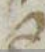
\includegraphics[height=1.5cm]{datapaper/images/examples/con/con_Sorbonne193.png}
            }
            \\
        \symbol{"2248} & U+2248 & esse &
            \raisebox{-.5\height}{%
            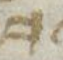
\includegraphics[height=1.5cm]{datapaper/images/examples/esse/esse_Sorbonne193.png}
            }
            \\
        ÷ & U+00F7 & est/id est &
            \raisebox{-.5\height}{%
            
\includegraphics[height=1.5cm]{datapaper/images/examples/est-idest/enim_est_2_MsWettF 15.png}
            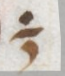
\includegraphics[height=1.5cm]{datapaper/images/examples/est-idest/enim_est_MsWettF 15.png}
            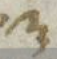
\includegraphics[height=1.5cm]{datapaper/images/examples/est-idest/enim_est_Sorbonne193.png}
            }
            \\
        \multirow{2}{*}{\symbol{"F1AC}} & U+F1AC & \multirow{2}{*}{-que/-bus/-m/-et} &
        
            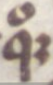
\includegraphics[height=1.5cm]{datapaper/images/examples/que/-que_CML13027.png}
            
\includegraphics[height=1.5cm]{datapaper/images/examples/que/que_2_Latin6395.png}
            
\includegraphics[height=1.5cm]{datapaper/images/examples/que/que_2_Phil10a135.png}
            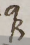
\includegraphics[height=1.5cm]{datapaper/images/examples/que/que_CCCC165n.png}
            \includegraphics[height=1.5cm]{datapaper/images/examples/que/que_egerton821.png}
            \includegraphics[height=1.5cm]{datapaper/images/examples/que/que_Latin 16195.png}
            \\ % Multi Rows
         & & &
            \includegraphics[height=1.5cm]{datapaper/images/examples/que/que_Latin6395.png}
             \includegraphics[height=1.5cm]{datapaper/images/examples/que/que_Laurentianus39.34.png}
            \includegraphics[height=1.5cm]{datapaper/images/examples/que/que_Montpelier.H 318.png}
            \includegraphics[height=1.5cm]{datapaper/images/examples/que/que_Phil10a135.png}
            \includegraphics[height=1.5cm]{datapaper/images/examples/que/que_Plut 53.08.png}
            \includegraphics[height=1.5cm]{datapaper/images/examples/que/que_Plut.53.09.png}
            \includegraphics[height=1.5cm]{datapaper/images/examples/que/que_VatLat373.png}
            \\
        \symbol{"A775} & U+A775 & -rum & 
            \raisebox{-.5\height}{%
            \includegraphics[height=1.5cm]{datapaper/images/examples/-rum/-rum_CML13027.png}
            \includegraphics[height=1.5cm]{datapaper/images/examples/-rum/rum_Plut 53.08.png}
            \includegraphics[height=1.5cm]{datapaper/images/examples/-rum/-rum_egerton821.png}
            \includegraphics[height=1.5cm]{datapaper/images/examples/-rum/-rum_MsWettF 15.png}
            \includegraphics[height=1.5cm]{datapaper/images/examples/-rum/-rum_Phil10a135.png}
            \includegraphics[height=1.5cm]{datapaper/images/examples/-rum/-rum_Latin 16195.png}
            }           
    \\ \hline
    \end{tabular}%
    }}
    \caption{Freestanding, letter-combining abbreviations and their corresponding transcription signs. \symbol{"0111} cannot be found in our dataset and is mentioned here as it might be a common case in other dataset.}
    \label{tab:all_abbr}
\end{table}

\textbf{Ligatures}, \textit{ie.} combinations of more than two letters in one form with the reduction of proclitic and enclitic letters or abbreviating symbols placed above or joined with letters are reduced to their original alphabetical components. Ligatures between letters in cursive scripts such as the \juni{\symbol{"FB05}} (U+FB05) ligature or the two \juni{\symbol{"FB00}} (U+FB00) ligature are resolved as -\textit{st}- and -\textit{ff}-. For the very frequent \textit{quia}, the transcription \textit{qr} has been privileged , avoiding the MUFI sign \juni{\symbol{"E8B3}} that belongs to the private domain. More examples are provided in the Table \ref{tab:all_lig}.\footnote{Other transcription guidelines privilege ``q2'' as a reference to the ``r rotunda-shaped'' abbreviation sign that lays next to q the choice of \textit{qr} from our part being the reduction to the r rotunda-shaped abbreviation sign to the simpler r. The original insular abbreviation has a simple vertical tilde next to the letter ``q''.}

\begin{table}[H]
    \centering
    \resizebox{\linewidth}{!}{%}
    {\junicodeFont%
    \begin{tabular}{c|c|c|c|c}
        \hline
        Type & Transcription & Unicode & Description or resolution & Examples \\ \hline
        \multirow{2}{*}{Ligature} & \multirow{2}{*}{st} & \multirow{2}{*}{-} & \multirow{2}{*}{Normally transcribed ligature} & 
         \raisebox{-.5\height}{
            \includegraphics[height=1.5cm]{datapaper/images/examples/st/st_Latin8236.png}
         }
         \\
         \textbf{Ligature} & .n. & - & \textit{enim} &
         \raisebox{-.5\height}{%
             \includegraphics[height=1.5cm]{datapaper/images/examples/enim_Montpelier.H 318.png}
            \includegraphics[height=1.5cm]{datapaper/images/examples/enim_Phil10a135.png}
        }
        \\
        \textbf{Ligature} & qr & - & \textit{quia} &
         \raisebox{-.5\height}{%
            \includegraphics[height=1.5cm]{datapaper/images/examples/quia/quia_Montpelier.H 318.png}
            \includegraphics[height=1.5cm]{datapaper/images/examples/quia/quia_MsWettF 15.png}
            \includegraphics[height=1.5cm]{datapaper/images/examples/quia/quia_Sorbonne193.png}
        }    
        \\
        \textbf{Monogrammatic Ligature} & qd & - & \textit{quod} &
         \raisebox{-.5\height}{%
            \includegraphics[height=1.5cm]{datapaper/images/examples/quod-Et/quod_Montpelier.H 318.png}
            \includegraphics[height=1.5cm]{datapaper/images/examples/quod-Et/quod_egerton821.png}
        }
        \\
                \textbf{Monogrammatic ligature} & Et & - & \textit{Et} &
         \raisebox{-.5\height}{%
            \includegraphics[height=1.5cm]{datapaper/images/examples/quod-Et/Et_Montpelier.H 318.png}
            }
        \\
        Contraction & aũt̃  & -  &Long vertical tilde transcribed by two tildes & 
        \raisebox{-.5\height}{
            \includegraphics[height=1.5cm]{datapaper/images/examples/extended_macron/double_macron_CML13027.png}
        }
        \\
        Contraction & ẽẽ & - & Long vertical tilde transcribed by two tildes \footnote{Instead of using the existing \juni{035E} or \juni{0360} than can be combined over two letters} ; & 
        \raisebox{-.5\height}{
            \includegraphics[height=1.5cm]{datapaper/images/examples/extended_macron/double_macron_egerton821.png}
            \includegraphics[height=1.5cm]{datapaper/images/examples/extended_macron/double_macron_Latin 16195.png}
        }
        \\
         Contraction & tp̃̃a & - & Two stacked tildes & 
        \raisebox{-.5\height}{
            \includegraphics[height=1.5cm]{datapaper/images/examples/extended_macron/superposed_macron_CML13027_bis.png}
        }
    \\ 
    \hline

      \end{tabular}
    }}
    \caption{\label{tab:all_lig}Ligatures and special contraction cases.}
\end{table}

\paragraph{Superscripts letters and interlinear additions} A standard way of contracting a word is by adding a superscript letter which gives information about the abbreviated sequence. Frequent ones are open a, u, o, or the ending of a word altogether. These were all rendered with the aid of superscript characters available in MUFI \cite[p. 11]{pinche:hal-03697382}. \textit{Ergo} and \textit{igitur} are two of the most frequent example of abbreviation with superscript letters. Letters without any baseline letter are simply represented with the same combining superscript character and a space as the supporting baseline character (\textit{e.g.}  \enquote{\juni{\symbol{"2007}\symbol{"0363}\symbol{"2007}\symbol{"036D}}}: space + combining a + space + combining t).

\begin{figure}[H]
    \centering
    \begin{subfigure}{0.30\linewidth}
    \centering
    \includegraphics[height=1.5cm]{datapaper/images/examples/superscripts/BIS193_bis.png}
    \end{subfigure}
    \begin{subfigure}{0.30\linewidth}
    \centering
    \includegraphics[height=1.5cm]{datapaper/images/examples/superscripts/CML13027.png}
    \end{subfigure}
    \begin{subfigure}{0.30\linewidth}
    \centering
    \includegraphics[height=1.5cm]{datapaper/images/examples/superscripts/montpelier_H318.png}
    \end{subfigure}  
    \begin{subfigure}{0.20\linewidth}
    \centering
    \includegraphics[height=1.5cm]{datapaper/images/examples/superscripts/montpelier_H318_bis.png}
    \end{subfigure}
    \begin{subfigure}{0.30\linewidth}
    \centering
    \includegraphics[height=1.5cm]{datapaper/images/examples/superscripts/BAV_pallat_373.png}
    \end{subfigure}
     \begin{subfigure}{0.30\linewidth}
    \centering
    \includegraphics[height=1.5cm]{datapaper/images/examples/superscripts/BIS193.png}
    \end{subfigure}
    \caption{\label{tab:superscript} Examples of contraction use of superscript letters.Manuscripts in the following order: BIS193, CML13027, Montpelier H-318, Montpelier H-318, BAV Pal. lat.373, BIS193.}
\end{figure}

A special case where superscript letters were used with a non-abbreviating function in the project and merits to be mentioned was for the transcription of interlinear additions. Especially in manuscripts with scholastic and medical content, missing words/explanations are added in the interlinear space, something which was at first a challenge for the transcription process due to segmentation constraints. More specifically, it can be, at times, impossible to completely differentiate the segmentation masks of two words that are very close to each other on the vertical axe (like the interlinear additions). Therefore, provided that the corresponding combining letter exists and both words can be formulated, no new lines were carved for the interlinear additions. Where this was deemed too complex, interlinear additions were omitted (see Figure \ref{interlinear}).

\begin{figure}[H]
    \centering
    \begin{subfigure}{0.20\linewidth}
    \centering
    \includegraphics[height=1.5cm]{datapaper/images/examples/superscripts/CML13027_bis.png}
    \end{subfigure}
    \begin{subfigure}{0.20\linewidth}
    \centering
    \includegraphics[height=1.5cm]{datapaper/images/examples/superscripts/CML13027_corr.png}
    \end{subfigure}
        \begin{subfigure}{0.20\linewidth}
    \centering
    \includegraphics[height=1.5cm]{datapaper/images/examples/superscripts/CML13027_crisis.png}
    \end{subfigure}
    \caption{All examples come from the CML 13027 manuscript.}
    \label{interlinear}
\end{figure}

\paragraph{Rare characters and Numerals}
\label{special_chars}

Referring to corpus construction practices for balanced corpora, \cite{maniaci1993che} stresses that \enquote{sporadically attested variables will therefore be preferred to those that appear in all - or almost all - the individuals that are part of the corpus.} Rare characters, a subset of freestanding abbreviation signs, specifically occurring in the Medii Aevi dataset are therefore given special attention. In two of the manuscripts, both of medical content, some occurrences of graphemes for the denotation of the metric values \textit{ounce} and \textit{semuncia} were encountered. For their transcription, the MUFI characters \juni{\symbol{"2125}} (U+2125) and \juni{\symbol{"10192}} (U+10192) were used. The character \enquote{barred O} is represented by the Unicode codepoint \juni{\symbol{"2205}} (U+2205, mathematical representation of an empty set) and is widely used to transcribe the word \textit{instans} instead of the \juni{\symbol{"A74B}} (U+A74B) that, according to MUFI recommendation stands for the abbreviation of \textit{obi(i)t} \cite[p.~10]{coulson2020oxford}.

\begin{table}[H]
    \centering
    \resizebox{\linewidth}{!}{%}
    {\junicodeFont%
    \begin{tabular}{c|c|c|c|c}
        \hline
        Type & Transcription & Unicode & Description or resolution & Examples \\ \hline
        \multirow{2}{*}{Symbols} & \multirow{2}{*}{\symbol{"2125}} & \multirow{2}{*}{U+2125} & \multirow{2}{*}{Ounce} & 
         \raisebox{-.5\height}{
            \includegraphics[height=1.5cm]{datapaper/images/examples/ounces/ounce_Montpelier.H 318.png}
            \includegraphics[height=1.5cm]{datapaper/images/examples/ounces/ounce_Phi10a135.png}
         }
        \\
        Symbols & \symbol{"10192} & U+10192 & *Semi-Ounce &
        \raisebox{-.5\height}{%
            \includegraphics[height=1.5cm]{datapaper/images/examples/ounces/semi_ounce_Phi10a135.png}
        }
        \\
        Abbreviations & \symbol{"2205} & U+2205 & \textit{instans} &
        \raisebox{-.5\height}{%
            \includegraphics[height=1.5cm]{datapaper/images/examples/instans/instans_Sorbonne193.png}
        }
             \\ \hline
    \end{tabular}
    }}
    \caption{Rare characters found in Montpellier H318, Phil., Col. of Phys. 10a 135 and BIS 193.}
\end{table}

Last but not least, in addition to roman numerals, which are fairly frequent in medieval manuscripts and in the CREMMA Medieval dataset, often preceded and followed by dots such as \enquote{.ii.}, Arabic numerals are also comprised in the dataset, mainly due to the medical treatises (see Figures \ref{fig:numerals} and  \ref{fig:numerals2}).\footnote{An excellent article dealing with numerals in Latin manuscripts is \cite{charles_numerals}.}
\begin{figure}[H]
    \centering
    \begin{subfigure}{0.20\linewidth}
    \centering
    \includegraphics[height=1.5cm]{datapaper/images/examples/numerals/arabic_4_Latin 16195.png}
    \end{subfigure}
    \begin{subfigure}{0.20\linewidth}
    \centering
    \includegraphics[height=1.5cm]{datapaper/images/examples/numerals/arabic_4_Phi10a135.png}
    \end{subfigure}
     \begin{subfigure}{0.20\linewidth}
    \centering
    \includegraphics[height=1.5cm]{datapaper/images/examples/numerals/arabic_9_Phi10a135.png}
    \end{subfigure}
    \begin{subfigure}{0.20\linewidth}
    \centering
    \includegraphics[height=1.5cm]{datapaper/images/examples/numerals/arabic_numeral_Phi10a135.png}
    \end{subfigure}
    \begin{subfigure}{0.20\linewidth}
    \centering
    \includegraphics[height=1.5cm]{datapaper/images/examples/numerals/arabic_sequence_Sorbonne193.png}
    \end{subfigure}
    \begin{subfigure}{0.20\linewidth}
    \centering
    \includegraphics[height=1.5cm]{datapaper/images/examples/numerals/roman_numeral_CML13027.png}
    \end{subfigure}
    \begin{subfigure}{0.20\linewidth}
    \centering
    \includegraphics[height=1.5cm]{datapaper/images/examples/numerals/roman_numeral_egerton821.png}
    \end{subfigure}  
    \begin{subfigure}{0.20\linewidth}
    \centering
    \includegraphics[height=1.5cm]{datapaper/images/examples/numerals/roman_numeral_Latin6395.png}
    \end{subfigure}
    \caption{Manuscripts in the following order: Latin 16195, Phi. 10 a. 135 (x3), BIS 193, CML13027, Egerton 821, Latin 6395.}
    \label{fig:numerals}
\end{figure}

%eventually a bit redundant but I wouldn't be able to tell the numbers without a reference?
\begin{figure}[H]
    \centering
    \includegraphics[width=1.5cm,angle=90]{datapaper/images/examples/numerals/BnF, lat.15461, fol.13r.jpeg}
    \caption{Snippet of Arabic numerals from BnF, lat.15461, fol.13r for comparison purposes.}
    \label{fig:numerals2}
\end{figure}

\paragraph{Production pipeline}

The data was built using eScriptorium and Kraken for both segmentation of zones and lines (specifically the BLLA model). Manuscripts were annotated successively. First, the manuscript is automatically segmented, then its segmentation is manually corrected (addition, deletion, and modifications), and the text is transcribed. Once each sample is entirely annotated, its use of characters is controlled via the ChocoMufin software, while its conformity to the segmentation classification vocabulary is controlled by HTRVX. Finally, data are released on Github.\footnote{\url{https://github.com/htr-united/cremma-medieval-lat}.}

All the combining and abbreviation signs suggested for use by the present adaptation of Old French guidelines can be also found on the custom-made Unicode keyboard, which can be imported in the \textit{eScriptorium} interface, conceived in order to facilitate and accelerate the transcription process and compatibility with the Unicode recommendations.\footnote{Available here: \url{https://github.com/HTR-United/CREMMA-Medieval-LAT/blob/main/keyboard.json}.}

\section{Results and discussion}

\paragraph{Properties of the resulting dataset}

The resulting version of the dataset (see Table \ref{tab:dataset}) is built on 18 + 3 manuscripts. All alignments are original alignments, but some draw their original transcription from online projects (\textit{cf.} Acknowledgements).

The current version of the dataset shows a wide variety of genres, and thus vocabulary. From medical and grammatical content to literary and scholastic a certain level of arbitrariness is introduced in the sequence of characters as they are not as repetitive and predictable from the machine as in a homogeneous genre or topic-driven dataset. The collection was built as to be not representative of one specific use of the Latin language and is not thematically unified - while the CREMMA Medieval dataset focuses more on literary texts, specifically hagiographic and \textit{chanson de geste} texts. %\footnote{\citet{bauer2000corpus}[p.30] \enquote{One may distinguish general-purpose corpora from topical corpora. A general-purpose-corpus is designed with a broad range of applications and research questions in mind and serves as a resource in the widest sense [...] the selection aims at balancing different registers to enable comparative research. It does not aim to be 100\% representative}.}.
Medical and scholastic genres, furthermore, induce the use of a range of rare characters and often underrepresented letters (such as \enquote{z} (zeta) and \enquote{y} (upsilon), as well as some rare \enquote{k} (kappas)).

Other features, such as layout and type of digitization (microfilm or original), provides different representations of texts, with more or less noise in the mask of each line given the space between them, with more or less contrast between information (colored text yields less \enquote{information} in digitized manuscripts as they tend to be a duller form of grey that black ink, while clearly departing from the manuscript \enquote{background} in color).

A time span of 5 centuries between the earliest and the oldest manuscripts, with a clear focus on the period starting in the 1200s and finishing in 1500. This leads to a good representation of a variety of Gothic scripts,\footnote{Characterisation of scripts was made by the transcriber where the information was not available on the notice of the manuscript. The criteria followed for the Gothic scripts are those of \cite{derolez2003palaeography}. %Thanks to professor Marc Smith and Dominique Stutzmann for their help in the identification process
} including personal hands alongside formal categories,\footnote{For the particular case of the \enquote{scritture di dotti}, or the distinctive scripts of scholars which do not wholly conform to Delorez' classification criteria, see the contribution of Maria Christina Rossi (Univ. of Pisa) at the 22\textsuperscript{nd} edition of CIPL (September 2022) \url{https://cipl.hypotheses.org/maria-cristina-rossi-univ-pisa}.} with different levels of execution (cursivity and formality). We note an intra-manuscript variation for letters such as single and two-compartment or open and closed s normal present in the same manuscript.


\begin{table}[H]
\centering
\resizebox{\columnwidth}{!}{%
\begin{tabular}{|l|rrrrrrr|}
\hline
Shelfmark ID                 & Pages & Type   & Date      & Status    & Script                     & Folio Sampling  & degree of abbreviations \\ \hline
Egerton 821                  & 4    & Medic. & 1100-1199 & Color     & Praegothica                 & Sequential      & medium                  \\  \hline
Montpellier H318             & 5    & Medic. & 1100-1299 & Color     & Semitextualis Libraria      & Sequential      & high                    \\ 
CCCC MSS 236                 & 5    & Lit.  & 1200-1225 & Color     & Textualis Libraria          & Sequential      & medium                  \\ 
CLM 13027                    & 5    & Medic. & 1250-1299 & Color     & Southern Textualis Libraria & Sequential      & high                    \\ 
Latin 16195                  & 4    & Medic. & 1250-1299 & Microfilm & Semitextualis Currens       & Sequential      & high                    \\ 
† MsWettF 15                 & 5    & Schol. & 1270-1280 & Color     & Textualis Libraria          & Sequential      & high                    \\ \hline
Laur. Plut. 33.31            & 5    & Lit.  & 1300-1310 & Color     & Textualis Meridionalis      & Sequential      & low                     \\ 
Arras 861                    & 5    & Lit.  & 1300-1399 & Color     & Textualis Formata           & Sequential      & medium                  \\ 
† BIS 193                    & 5    & Schol. & 1300-1399 & Color     & Textualis currens           & Sequential      & high                    \\ 
Phil., Col. of Phys. 10a 135 & 5    & Medic. & 1300-1399 & Color     & Cursiva recentior           & Sequential      & medium                  \\ 
† Mazarine Ms. 915           & 4    & Schol. & 1300-1399 & Color     & Textualis Meridionalis      & Sequential      & high                    \\ 
‡ UBL, Ms 758                & 15   & Eccl.  & 1320-1340 & Color     & Textualis Libraria          & Semi-Sequential & low                     \\
Latin 6395                   & 6    & Lit.  & 1325-1399 & Microfilm & Semitextualis Libraria      & Sequential      & low                     \\ \hline
Laur. Plut. 39.34            & 5    & Lit.  & 1400-1499 & Color     & Humanistica Cursiva         & Sequential      & low                     \\ 
† Vat. Pal. Lat. 373         & 4    & Schol. & 1400-1499 & Microfilm & Hybrida Currens             & Sequential      & low                     \\ 
Laur. Plut. 53.08            & 4    & Gramm. & 1459      & Color     & Personal Humanistica        & Sequential      & medium                  \\ 
Laur. Plut. 53.09            & 4    & Gramm. & 1400-1499 & Color     & Humanistica Rotunda         & Sequential      & low                     \\ 
‡ Berlin, Hdschr. 25         & 17   & Eccl.  & 1400-1499 & Color     & Textualis Formata           & Semi-Sequential & low                     \\
‡ Berlin, Germ. Oct. 511     & 6    & Eccl.  & 1400-1499 & Color     & Hybrida formata             & Semi-Sequential & low                     \\
Latin 8236                   & 5    & Lit.  & 1471-1499 & Microfilm & Humanistica Cursiva         & Random          & low                     \\ \hline
† CCCC MSS 165               & 5    & Schol. & 1500-1599 & Color     & Personal Cursive            & Sequential      & medium                  \\ \hline
\end{tabular}%
}
\caption{Basic features and length of the dataset in chronological order. Medic. stands for medical, Lit. for literature, Schol. for scholastic commentaries, Gramm. for grammatical commentaries, Eccl. for church literature (book of hours, psalms, etc.). Texts preceded by a ‡ are aligned and corrected using the Berlin Transcribathon dataset, by a † using the SCTA TEI editions.}
\label{tab:dataset}
\end{table}

\paragraph{Character frequencies in the CREMMA Medieval and the Medii Aevi datasets} We set up this corpus to both complement the CREMMA Medieval dataset and grow the available set of data for Latin through the Middle Ages, noting that at least two datasets for Medieval Latin existed already (Caroline Minuscule and Eutyches) in abbreviated form for pre-10th century documents.

\begin{table}[H]
    \centering
    {\junicodeFont%
    \begin{tabular}{ll|rr|rr}
    \hline
    Character  & Unicode &    Latin &  Old French & \% in Latin & Ratio \\
    \hline
    \symbol{"204A} &       U+204A &  2228.0 &      4400.0 &              33.61 &   0.51 \\
    \symbol{"036C} &       U+036C &   148.0 &       219.0 &              40.33 &   0.68 \\
    \symbol{"0026} &       U+0026 &    83.0 &       116.0 &              41.71 &   0.72 \\ \hline
    \symbol{"A76F} &       U+A76F &   850.0 &       779.0 &              52.18 &   1.09 \\ \hline
    \symbol{"A751} &       U+A751 &  1500.0 &       919.0 &              62.01 &   1.63 \\
    \symbol{"0365} &       U+0365 &  1486.0 &       820.0 &              64.44 &   1.81 \\
    \symbol{"0303} &       U+0303 & 14445.0 &      5759.0 &              71.50 &   2.51 \\
    \symbol{"0363} &       U+0363 &  2024.0 &       732.0 &              73.44 &   2.77 \\
    \symbol{"A770} &       U+A770 &  1763.0 &       523.0 &              77.12 &   3.37 \\
    \symbol{"033E} &       U+033E &  3827.0 &       973.0 &              79.73 &   3.93 \\
    \symbol{"0364} &       U+0364 &   518.0 &       120.0 &              81.19 &   4.32 \\
    \symbol{"A753} &       U+A753 &   462.0 &        80.0 &              85.24 &   5.78 \\
    \symbol{"1DD1} &       U+1DD1 &  1018.0 &       137.0 &              88.14 &   7.43 \\
    \symbol{"1DE4} &       U+1DE4 &   978.0 &        55.0 &              94.68 &  17.78 \\
    \symbol{"0366} &       U+0366 &   870.0 &        61.0 &              93.45 &  14.26 \\
    \hline
    \end{tabular}
    }
    \caption{Abbreviating signs, present more than 50 times in both the Latin and the Old French CREMMA datasets. The CREMMA Medieval (Old French) dataset is comprised of 693,052 characters in total, which makes it more than twice the size of CREMMA Medii Aevi. Despite this difference, most abbreviated characters are more represented in the Latin dataset.}
    \label{tab:chars}
    \normalfont
\end{table}

Unlike CREMMA Medieval, our approach has been feature-driven, as we tried, as much as possible, to find data that would ultimately allow for better recognition of special characters outside the classical A-Z range. In this regard, we succeeded, as we have a higher frequency of MUFI or special characters in our dataset than in the Medieval Old French dataset, despite being smaller overall (see Table \ref{tab:chars}). Only three characters are more represented in the other dataset: the Tironian Et, the superscript combining R (common on words such as \enquote{grand} [large, big]), and the ampersand \&. The character \juni{ꝯ} is equally present in both datasets: resolved as con- or com- in French, it is often used in words such as \juni{ꝯmence} (\textit{commence}, to start). Some very frequent diacritics, such as the horizontal lines and vertical lines (transcribed in vertical or horizontal tildes according to Pinche's guidelines), have seen a rise in presence: horizontal tildes are 2.51 times more seen in our Latin corpora, and the vertical tilde 3.93. This will allow better recognition of these two frequent marks, as it now totals around 19,000 occurrences in both datasets for the horizontal tilde and 4,500 for the vertical one, making them the first and the third most represented abbreviating characters in the CREMMA-funded datasets.

Overall, our dataset presents texts that are more varying in terms of features than the Old French dataset (see Figure \ref{fig:char_freqs_mss}). This is the result of our feature-driven approach. However, some manuscripts have nearly no abbreviation, Laur. Plut. 39.34 notably so as it only contains 3 abbreviated words which is a single character abbreviation (\juni{⁊}, \textit{et}). A little less than half of our manuscripts are less abbreviated than the most abbreviated text in the CREMMA Medieval dataset, while the other half can beat it with up to ten points. However, both languages show similar maximum frequencies in terms of non-single letter abbreviations (abbreviations made up of a single character in MUFI such as \juni{⁊, \&, ꝑ}).\footnote{This definition, while useful to quantify some phenomenon, is debatable and should not be used to make a quantitative conclusion on these languages, they merely inform us about our dataset. For example, etiam (\juni{⁊} + tilde) is technically a single letter with a diacritic, but will be counted as two characters in our case.} 

Finally, despite showing a similar number of \textit{pages}, we see a large variation in terms of word density with a somewhat limited variation in terms of unique words. This shows how pages as a metric are not enough to characterize a corpus for HTR and Layout segmentation purposes: the number of columns, lines, and potentially of words or characters supplements the first. To showcase this argument, the Berlin, Hdschr. 25 manuscript has the highest number of pages (17) but the third lowest amount of words (961).

\begin{table}[]
    \centering
    \resizebox{\linewidth}{!}{%}
\begin{tabular}{ll|rrrrr}
\hline
      Lang &     type &     Words  &   Words \% &  Unique words  &  Unique words \% &  Freq. of unique words > 1 \\
\hline
     Latin &   abbr.  &   6,855 &  11.94\% &          1,460 &           6.24\% &                   279 \\
     Latin &  others  &  50,557 &  88.06\% &         21,935 &          93.76\% &                  5,025 \\
Old French &   abbr.  &   5,755 &   4.15\% &          1,457 &           4.89\% &                   286 \\
Old French &  others  & 132,828 &  95.85\% &         28,315 &          95.11\% &                  8,726 \\
\hline
\end{tabular}
}
\caption{Comparative statistics table on abbreviations: for each dataset, we look at words that are abbreviated (abbr.) or non-abbreviated (others). It reads the following way: \enquote{11.94\%}}
\label{tab:abbr-fro-lat}    
\end{table}

\begin{table}[]
    \centering
\resizebox{\linewidth}{!}{%
\begin{tabular}{lrrrrrrrr}
\hline
Manuscript &  Words &  Un. Words &  Abbr. words &  Abbr. ratio &  \textit{NSCA} &  \textit{NSCA} ratio &  Un. abbr. &  Un. abbr. ratio \\
\hline
Laur. Plut. 39.34            &    783 &           571 &                  3 &        0.38\% &       0 &       0.00\% &             1 &               0.18\% \\.
Berlin, Germ. Oct. 511       &    \textbf{171} &           134 &                 1   &        0.58\% &       0 &       0.00\% &             1 &               0.75\% \\
Berlin, Hdschr. 25           &    961 &           654 &                 12 &        1.25\% &           3 &       0.31\% &             6 &               0.92\% \\
Latin 8236                   &   1475 &          1057 &                 33 &        2.24\% &           5 &       0.34\% &             6 &               0.57\% \\
Laur. Plut. 33.31            &   1278 &           858 &                 36 &        2.82\% &          17 &       1.33\% &            21 &               2.45\% \\
Laur. Plut. 53.09            &   1300 &           798 &                 38 &        2.92\% &          10 &       0.77\% &             9 &               1.13\% \\
CCCC MSS 165                 &   1521 &           713 &                 49 &        3.22\% &          28 &       1.84\% &            23 &               3.23\% \\
CCCC MSS 236                 &   1239 &           874 &                 68 &        5.49\% &          44 &       3.55\% &            24 &               2.75\% \\
Latin 6395                   &   3304 &          2418 &                190 &        5.75\% &          85 &       2.57\% &            72 &               2.98\% \\
Laur. Plut. 53.08            &   2985 &          1870 &                195 &        6.53\% &          94 &       3.15\% &            67 &               3.58\% \\ \hline
UBL, Ms. 758                 &   4468 &          2393 &                297 &        6.65\% &          72 &       1.61\% &            64 &               2.67\% \\
Arras 861                    &   2416 &          1601 &                164 &        6.79\% &         101 &       4.18\% &            80 &               5.00\% \\
Egerton 821                  &    981 &           677 &                 71 &        7.24\% &          28 &       2.85\% &            31 &               4.58\% \\
Phil., Col. of Phys. 10a 135 &   1487 &          1057 &                151 &       10.15\% &          52 &       3.50\% &            44 &               4.16\% \\
Montpellier H318             &   4456 &          2316 &                458 &       10.28\% &         131 &       2.94\% &           109 &               4.71\% \\
Vat. Pal. Lat. 373           &   2258 &          1203 &                234 &       10.36\% &          69 &       3.06\% &            67 &               5.57\% \\
Latin 16195                  &   4135 &          1676 &                569 &       13.76\% &         168 &       4.06\% &           107 &               6.38\% \\
MsWettF 15                   &   3574 &          1452 &                501 &       14.02\% &         172 &       4.81\% &           107 &               7.37\% \\
CLM 13027                    &   6499 &          3612 &                970 &       14.93\% &         340 &       5.23\% &           257 &               7.12\% \\
BIS 193                      &   \textbf{7370} &          2731 &               1161 &       15.75\% &         413 &       5.60\% &           244 &               8.93\% \\
Mazarine Ms. 915             &   4751 &          1873 &                824 &       17.34\% &         350 &       7.37\% &           195 &              10.41\% \\
\hline
\end{tabular}
%
}
    \caption{Statistics per manuscript. \enquote{Un.} stands for Unique, \enquote{Abbr.} for Abbreviated or Abbreviation, \enquote{NSCA} for Non-Single Character Abbreviation. The lowest and highest values are in bold typeface. The separation between Laur. Plut. 53.08 and UBLMs. 758 represents the highest abbreviation ratio in the CREMMA Medieval dataset.}
    \label{tab:mss_words}
\end{table}



\begin{figure}
    \centering
    \includegraphics[width=.8\linewidth]{datapaper/images/figures/type_freq.png}
    \caption{Frequences of character classes across manuscripts}
    \label{fig:char_freqs_mss}
\end{figure}

\section{Implications/Applications}

With this addition to the overall amount of datasets available, we now have 1.149 million characters for Medieval manuscripts with book scripts, ranging from the 9th to the 15th century. These data offer more than characters, as we can imagine using them in the context of linguistic studies (evolution of dialects, abbreviation usage, etc.) thanks to the common transcription norm or in codicology studies (evolution of layouts, relation between layouts) thanks to the common segmentation vocabulary, both using the original data or automatically annotated one.

As a direct output, we trained a model which would allow for transcribing or starting the transcription of Latin medieval manuscripts. In order to evaluate the gain from our data, we trained three models:
\begin{enumerate}
    \item a model containing all data from the Table \ref{tab:datasets}, to help transcribe Latin and Medieval French manuscripts, which is the end goal of this paper;
    \item a model containing every dataset but our own, to evaluate the impact regarding the quantity of data we add for Latin (\textit{i.e.}, to find out if the original Carolingian datasets were enough to break the language model of the Old French datasets);
    \item a model containing only Old French data, from \textit{incunabula} of the 15th century to the main dataset CREMMA Medieval.
\end{enumerate}
Each model uses at least 10\% of the pages of each dataset for the development set. CREMMA Medieval and CREMMA Medii Aevi are split furthermore with another 10\% subset for evaluation, proposing \enquote{In Domain} evaluation. From CREMMA Medii Aevi, as stated earlier, all aligned data from the \textit{Faithful Transcription Data Set} are kept for testing, as an out-of-domain set.

The results show a massive improvement for the in-domain Latin dataset (see Table \ref{tab:trainin-results}) and an insignificant one for Old French. The addition of the CREMMA Medieval Dataset provides overall better results on out-of-domain datasets from the three manuscripts taken into account, UBL Mss. 758 and Berlin, Hdschr. 25 display an improvement of 4.2 points at least (over around 30\% of CER) while Berlin, Germ. Oct. 511 (BGO), the smallest transcription set of the dataset, shows an improvement of below 2.4\%. This improvement derives equally from the simple addition of Latin into the model, as shown by the clear gap between the mixed model with Carolingian data: not only the model might benefit from Latin in general (as potentially shown by the simple addition of the Carolingian data), but it also gains in performance out of the amount of data from the same period as the generic Old French CREMMA Medieval dataset. We actually see in table \ref{tab:chars-errors} that there are much fewer errors on characters that saw their frequencies jump from a few thousand or hundreds of occurrences to many thousands one. The \textit{All} model does only a fourth of the error of the \textit{Only Old French} model on Tilde or two-thirds on vertical tildes for the UBL manuscript. The -rum abbreviation (\juni{ꝵ}) or the -et/-ed/-ibus one ( \juni{\symbol{"F1AC})} are quite new to the medieval datasets in general, which explains the clear difference in results. Overall, this dataset helped create a model allowing for readable output (see Table \ref{tab:diff-gt} for a side-by-side comparison) on medieval manuscripts, or at least transcription that can help produce new data.



\begin{table}[]
    \centering
    \resizebox{\linewidth}{!}{%}
    \begin{tabular}{llllll}
    \hline
    Model                       & Medieval Old French (In Domain) & Medieval Latin (In Domain) & UBL   & BGO   & BH25   \\ \hline
    All                         & 94.30        & 90.15                      & 71.69 & 79.12 & 85.10 \\
    No CREMMA Medii Aevi          & 94.04        & 80.68                      & 67.68 & 78.02 & 81.89 \\
    Only Old French                    & 94.01        & 78.10                      & 67.49 & 76.81 & 80.74 \\ \hline
    \end{tabular}
    }
    \caption{General accuracy results of the models. Model \textit{All} contains all data presented in Table \ref{tab:datasets}, model \textit{No CREMMA Medii Aevi} contains everything but the present dataset, model \textit{Only Old French} contains all datasets but Latin one (Eutyches, Caroline, CREMMA Medii Aevi). Two types of test sets are present: the \enquote{In Domain} dataset are pages from the same manuscripts as the models, all others (UBL 758, BGO 511, and B.H. 25) are manuscripts from the \textit{Faithful Transcriptions Data Set} aligned in CREMMA Medii Aevi but not used for training purposes.}
    \label{tab:trainin-results}
\end{table}

\begin{table}[]
    \centering
    \resizebox{\linewidth}{!}
\begin{tabular}[H]{ll|r|rrrrrrrrrrrrr}
   model & test &  [Space] \% & [Space] & Tilde &  Vert. Tilde &  7 &  ꝰ &  ꝯ &  ꝑ &  ħ &  ł &  ꝙ &  ꝓ &  ꝵ &  \symbol{"F1AC} \\
\hline 
     All           &  CREMMA Medieval &             1.7 &    803 &               77 &     46 &  0 & 10 & 17 & 15 &  0 &  0 &  0 &  4 &  0 &       0 \\
No CREMMA Medii Aevi &  CREMMA Medieval &             1.7 &    726 &               89 &     55 &  0 & 15 & 12 & 15 &  0 &  0 &  0 &  3 &  0 &       0 \\
   Only Old French        &  CREMMA Medieval &             1.7 &    733 &               86 &     50 &  0 & 12 & 15 & 20 &  0 &  0 &  0 &  2 &  0 &       0 \\ \hline
     All           &  CREMMA Medii Aevi &             1.7 &     74 &               27 &     31 &  0 &  3 &  2 &  3 &  0 &  8 &  2 &  2 &  0 &       1 \\
No CREMMA Medii Aevi &  CREMMA Medii Aevi &             2.8 &    138 &               78 &     92 &  0 & 17 &  8 & 11 &  1 & 17 & 15 &  2 & 15 &      32 \\
   Only Old French        &  CREMMA Medii Aevi &             3.1 &    149 &               91 &     87 &  0 & 16 & 10 &  9 &  1 & 17 & 20 &  2 & 15 &      33 \\ \hline
     All           &  BGO &             2.9 &     22 &                1 &      0 &  1 &  1 &  0 &  0 &  0 &  0 &  0 &  0 &  1 &       2 \\
No CREMMA Medii Aevi &  BGO &             2.3 &     13 &                3 &      0 &  1 &  1 &  0 &  0 &  0 &  0 &  0 &  0 &  1 &       2 \\
   Only Old French        &  BGO &             2.3 &     13 &                1 &      0 &  1 &  1 &  0 &  0 &  0 &  0 &  0 &  0 &  1 &       2 \\ \hline
     All           &  BH25 &             1.9 &     63 &               44 &     18 &  0 &  2 &  0 &  8 &  0 &  5 &  1 &  2 &  3 &      10 \\
No CREMMA Medii Aevi &  BH25 &             1.8 &     73 &               68 &     21 &  0 &  4 &  0 &  9 &  0 &  5 &  1 &  2 &  3 &      12 \\
   Only Old French        &  BH25 &             2.1 &    100 &               71 &     21 &  0 &  5 &  0 &  5 &  0 &  5 &  1 &  2 &  3 &      12 \\ \hline
     All           &  UBL &             4.4 &    274 &               67 &     48 &  0 & 12 &  0 & 54 & 10 & 30 &  2 & 14 & 30 &      43 \\
No CREMMA Medii Aevi &  UBL &             6.0 &    482 &              256 &     76 &  0 & 38 &  0 & 69 & 11 & 37 &  7 & 16 & 71 &      71 \\
   Only Old French        &  UBL &             5.7 &    484 &              239 &     77 &  0 & 28 &  0 & 59 & 11 & 37 &  7 & 15 & 71 &      71 \\ 
\end{tabular}
}}
    \caption{Details on errors from the test presented in Table \ref{tab:trainin-results}. Space \% shows the portion of error points due to bad spacing, \textit{e.g.} \textit{All} Model has a 94.30\% accuracy on CREMMA Medieval test set, which means a 5.7\% Character Error Rate (CER): not recognized SPACES represent 1.7 points of CER, more than a quarter of the CER. Other numbers are absolute values of missed characters (deletion or substitutions) to make comparisons between models possible; insertions are not accounted for.}
    \label{tab:chars-errors}
\end{table}

%\subsection{Resulting Model}

%\subsection{Abbreviation resolution as a secondary task}

\section*{Acknowledgements}

A number of transcriptions are the product of alignment and adaptation of existing projects that have worked on the manuscripts in question. In the case of existing digitized transcriptions, an alignment and correction were performed. In the case of printed editions, they served as a guide for obscure passages and \textit{dubia}.
\begin{itemize}
    \item For the manuscripts: MsWettF 15, BIS 193, Latin 6395, Vat. Pal. Lat. 373  and CCCC MSS 165, the transcriptions of Sentences Commentary Text Archive (SCTA) Project by Jeffrey C. Witt \citep{witt2016digital}.\footnote{The GitHub repository of the project can be found here: \url{https://github.com/scta-texts} and their reading room here: \url{https://scta.lombardpress.org/}} In the case of \textit{dubia}, additional corrections have been made for the faithful reproduction of the abbreviations ;
    \item for Berlin, Hdschr. 25, \textit{Faithful Transcriptions Data Set}  \citep{eichenberger_nicole_2021_5582483};
    \item for the Donatus manuscripts: Laurentianus Pluteus 53.08 and 53.09, the edition of HyperDonat by Bruno Bureau \& Christian Nicolas has been consulted \citep{bureau2008hyperdonat} and \citep{pinche2016hyperdonat}, preserving, nevertheless, the manuscript \textit{lectiones}/errors;
    \item In the same vein, for Latin 16195, the critical edition of \textit{Questiones de coitu} \citep{cartelle2017questiones}, for  Montpelier H 318 and CLM 1302, the critical edition of \textit{Liber minor de coitu} \citep{cartelle1987liberminor} and for Philadelphia, College of Physicians, 10a 135, the critical edition of the \textit{Tractatus de sterilitate} \citep{cartelle1993tractatus} by Enrique Montero Cartelle were consulted respectively as reference.
\end{itemize}


Tools used for verification of any \textit{dubia} in original transcriptions:
\begin{itemize}
    \item The online version of the Capelli: \url{https://www.adfontes.uzh.ch/fr/ressourcen/abkuerzungen/cappelli-online}
    \item During the deliberation regarding the use of special characters, the MUFI recommendations for Latin (last version) were respected \citep{wills2016medieval} available here: \url{https://folk.uib.no/hnooh/mufi/specs/MUFI-CodeChart-3-0.pdf}.
\end{itemize}


\section*{Funding Statement}

The project CREMMA was funded by the DIM MAP (now DIM PAMIR) under the supervision of the Conseil Régional d'Île de France. Part of the alignment of data for the \textit{Faithful Transcription Data Set} and the complete writing time for this paper was done under the funding of the second phase of CREMMALab post-doc (Thibault Clérice). The article publication fees are provided by the Centre Jean Mabillon.

\section*{Competing interests} 

The author(s) has/have no competing interests to declare.

\bibliographystyle{johd}
\bibliography{datapaper/biblio/mybibliography}

\section*{Appendix}

\begin{table}[H]
\resizebox{\linewidth}{!}{%}
{\junicodeFont
\begin{tabular}{rl|rl}
            \hline
            & Ground Truth & & Prediction \\ \hline
            1 & ouum faciet dñs suꝑ~\hl{t}erram. mulier ci\hl{r}cumdabit~\hl{v}i\hl{ꝵ} & 1 & ouum faciet dñs suꝑ~\hl{c}erram. mulier cicumdabit~\hl{u}i\hl{x aa-} \\
            2 & gremi\hl{o}~uteri sui~\hl{.I}eremie xxxi.~\hl{.V}ere nouũ fecit~\hl{doĩ}ꝰ & 2 & \hl{I~}gremi\hl{q}~uteri sui~\hl{J}eremie~\hl{.}xxx\hl{~.}i.~\hl{Is}ere\hl{̃}~nouũ fecit~\hl{an}ꝰ \\
            3 & \hl{⁊~}om\hl{ni}bus hominib~\hl{mi}rande~\hl{m}ult\hl{um~}.Et n\hl{o}ta in\hl{~annun}̃\hl{cc}iac\hl{o}̃ & 3 & \hl{I}o\hl{ns}mbus hominib~\hl{nu}rande~\hl{sis}ul\hl{cũ}t\hl{i}.\hl{~}Et n\hl{a}ta~\hl{ni am}in\hl{e}̃\hl{t}i\hl{~}ac̃\hl{i} \\
            4 & qd\hl{̾}~scd̾m tripli\hl{c}em terram t\hl{r}ia fecit dñs genera marie\hl{.} & 4 & qd\hl{̃}~scd̾m trip\hl{̃}li\hl{t}em terram t\hl{i}ia fecit dñs genera marie\hl{:} \\
            5 & nouo\hl{ꝵ D}i\hl{c}itur .\hl{ii}. terra bt̃a uirgo maria. terra dicitur ip & 5 & nouo\hl{r p}i\hl{t}itur .\hl{n}. terra bt̃a uirgo maria. terra dicitur ip \\
            6 & sa~\hl{c}iuitas bethleem\hl{~}.te\hl{r}ra di\hl{c}i\hl{᷑}~romanũ~\hl{i}mperiũ in\hl{~}qualib & 6 & sa~\hl{t}iuitas bethleem.\hl{~}te\hl{i~}ra di\hl{t}i romanũ mperiũ inqualib \\
            7 & istaꝵ ter\hl{r}a\hl{ꝵ}~fecit dñs nouũ~\hl{D}i\hl{c}~g\hl{ͦ N}o\hl{u}ũ faciet dñs~\hl{et}~cet\hl{er}a. & 7 & istaꝵ ter\hl{i~}a\hl{x}~fecit dñs nouũ~\hl{dd}i\hl{t}~g\hl{ͥ g}o\hl{n}ũ faciet dñs~\hl{⁊}~cet\hl{᷑}a. \\
            8 & \hl{D}e prima te\hl{rr}a in\hl{~}qua dñs fecit magna .i.~\hl{i}n\hl{~}bt̃a u\hl{̾}gine ma & 8 & \hl{d}e prima te\hl{ni}a inqua dñs fecit magna .i.~\hl{m}nbt̃a u\hl{ͥ}gine ma \\
            9 & ria di\hl{c}it pͣs.~\hl{B}ñdixisti dñe terram tuam. Vere bñdixit eã & 9 & ria di\hl{t}it pͣs.~\hl{b}ñdixisti dñe terram tuam\hl{i}. Vere bñdixit eã \\
            10 & deus mũdando ab\hl{~}orig\hl{i}nali pcc̃o\hl{.}~in\hl{~}u\hl{t}ero materno ipsam & 10 & deus mũdando aborig\hl{n}nali pcc̃o inu\hl{c}ero materno ipsam \\
            11 & scĩficando ⁊ ea\hl{m}~do\hl{n}is celestib\hl{u} replendo~\hl{| I}uxta i\hl{ll}ud~\hl{E}c\hl{̃}c̃.p\hl{t}ꝰ & 11 & scĩficando ⁊ ea\hl{ni}~do\hl{u}is\hl{̾}~celestib replendo~\hl{s}uxta i\hl{ł}ud~\hl{o}cc̃.\hl{~}p\hl{c}ꝰ \\
            12 & hec deus in\hl{~}terram aspe\hl{x}it ⁊ repleuit eam donis suis~\hl{D}eꝰ & 12 & hec deus interram aspe\hl{r}it ⁊ repleuit eam donis suis~\hl{d}eꝰ \\
            13 & b\hl{t}̃\hl{a}m ui\hl{r}gĩem donis~\hl{c}elestib repleuit quand\hl{o}~in\hl{~}eam de & 13 & b\hl{ca}̃m ui\hl{l.~}gĩem donis~\hl{t}elestib repleuit quand ineam de \\
            14 & scendit ⁊ ex\hl{~}ea deus ⁊ hom\hl{o}~nas\hl{c}i uolu\hl{i}t\hl{~}.\hl{v}nde sc̃a fuit an & 14 & scendit ⁊ exea deus ⁊ hom\hl{a}~na\hl{̃}s\hl{t}i uolu\hl{r}t.\hl{~u}nde sc̃a fuit an \\
            15 & teꝙͣ nata\hl{~}.prima e\hl{m}̃ terra .s. eua fuit maledicta ⁊ ideo~\hl{tr}i & 15 & teꝙͣ nata.\hl{~}prima e\hl{n}̃ terra .s. eua fuit maledicta ⁊ ideo~\hl{n}i \\
            16 & \hl{b}ulos ⁊ sp\hl{in}as~\hl{g}erminauit s hec terra est b\hl{t}̃a u\hl{̾}go ma & 16 & \hl{h}u\hl{̃}los ⁊ sp\hl{m}as~\hl{p}erminauit s hec terra est b\hl{r}̃a u\hl{ͥ}go ma \\
            17 & ria bñdicta\hl{~}.L\hl{u}ce\hl{~}.Bñdi\hl{c}ta tu in mulieribꝰ ⁊\hl{c}̾\hl{~V}n\hl{̃}~de ip̃a dicit\hl{᷑} & 17 & ria bñdicta.\hl{~}L\hl{i}ce.\hl{~}Bñdi\hl{t}ta tu in mulieribꝰ ⁊\hl{t}̾\hl{.v}n de ip̃a dici\hl{̃}t \\
            18 & Ecc\hl{ł}iastici .i\hl{ͦ}.~\hl{G}eneracio p\hl{̃}terit ⁊ gn̾acio aduenit terra~\hl{u}e & 18 & Ecc\hl{l}iastici .i.~\hl{E}eneracio p\hl{ͥ}terit ⁊ gn̾acio aduenit terra~\hl{ni}e \\
            19 & ro~\hl{in~}eternũ s\hl{t}at\hl{~.G}eneracio angeloꝵ p̃ter\hl{i}t fugiend\hl{o}~et & 19 & ro~\hl{m}eternũ s\hl{r}at\hl{i f}eneracio angeloꝵ p̃ter\hl{s}t fugiend et \\
            20 & credendo\hl{~}⁊ genera\hl{c}i\hl{o}~aduenit .s. latr\hl{o}~ꝯfitẽs xp̃\hl{m .}r\hl{̾}a uͦ & 20 & credendo\hl{.}⁊ gener\hl{~}a\hl{t}i\hl{a}~aduenit .s. latr\hl{a}~ꝯfitẽs xp̃\hl{u t̾}ra uͦ\hl{ͥ} \\
            21 & \hl{.}s.\hl{~}bt̃a u\hl{i}rgo in\hl{~}eter\hl{nũ}~stat .i. ꝑmansit ⁊ ꝑmanet ĩm\hl{o}bi & 21 & s.bt̃a~\hl{i}urgo ineter\hl{mt}~stat .i. ꝑmansit ⁊ ꝑmanet ĩ\hl{~}m\hl{a}bi \\
            22 & li\hl{s}~quia fundata erat suꝑ n\hl{i}chilũ pau\hl{ꝑ}tatis~\hl{.V}ñ iob fũ & 22 & li\hl{o}~quia fun\hl{̃}data erat suꝑ nchilũ pau\hl{p}tatis~\hl{u}ñ iob fũ \\
            23 & dauit terram suꝑ nichilum .s\hl{.}~hu\hl{i}ꝰ u̾gĩs pau\hl{ꝑ}t\hl{ati}s~\hl{Pa}u & 23 & dauit terram suꝑ nichilum .s hu\hl{r}ꝰ u̾gĩs pau\hl{p}t\hl{der}s~\hl{pd}u \\
            24 & \hl{ꝑ}tas eiu\hl{s}~patuit~\hl{|~}quan\hl{d}o~\hl{fi}liũ eius pannis~\hl{in}uoluit\hl{.} & 24 & \hl{p}tas eiu\hl{ã}~patuit quan\hl{t}o~\hl{a}liũ eius pannis~\hl{m}uoluit \\
            25 & In ha\hl{c}~terra ⁊ suꝑ han\hl{c}~terram fecit dñs multa noua et & 25 & In ha\hl{t}~terra ⁊ suꝑ han\hl{t}~terram fecit dñs multa noua et \\
            26 & p̃\hl{c}ipue qnͥq\hl{.|~}pͥmum no\hl{u}ũ qd̾ ꝯcepit deũ ⁊ hõiem~\hl{U}nde ꝓ & 26 & p̃\hl{t}ip\hl{̾}ue qnͥq\hl{~p}pͥmum\hl{̃}~no\hl{l}ũ qd̾ ꝯcepit deũ ⁊ hõiem~\hl{u}nde ꝓ \\
            27 & \hl{u}erbio\hl{ꝵ}~Diues ⁊ pauꝑ obuiauerũt sibi~\hl{D}iues ⁊ p\hl{a}u\hl{ꝑ}~deus & 27 & \hl{n}er\hl{~}bio\hl{r}~Diues ⁊ pauꝑ obuiauerũt sibi~\hl{d}iues ⁊ p\hl{d}u\hl{p}~deus \\
            28 & ⁊\hl{~}ho\hl{m}o obu\hl{i}auerũt sibi in utero u\hl{̾}gĩali~\hl{P}s\hl{ͣ h}o\hl{m}o natus & 28 & ⁊ho\hl{n}o obu\hl{l}auerũt sibi in utero ugĩali~\hl{pͥ}s\hl{. H}o\hl{ni}o natus \\
            29 & est in e\hl{a}~⁊c\hl{̾}~nõne magnũ nouũ ⁊ admirandũ oĩb quia\hl{~i}̃ & 29 & est in e\hl{s}~⁊c\hl{ͦ}~nõne magnũ nouũ ⁊ admirandũ oĩb quia\hl{t}̃ \\
            30 & virgĩ\hl{e y}ma sũmis sociant᷑\hl{.}~pater in\hl{~}filio qui oĩa cre\hl{a}uit & 30 & virgĩ\hl{t iͥ}ma sũmis sociant᷑ pater infilio qui oĩa cre\hl{d}uit \\
            31 & ex\hl{~}nichilo s\hl{o}lo uerbo ꝯ\hl{cl}udit᷑ in u\hl{̾}gĩs utero O qnͣta est benig & 31 & exnichilo s\hl{a}lo uerbo ꝯ\hl{d}udit᷑ in u\hl{ͥ}gĩs utero O qnͣta est benig\hl{̃} \\
            32 & nitas ⁊ h\hl{ũ}ilitas.\hl{~}regẽ uelle fieri ser\hl{u}ũ\hl{.}~panẽ a\hl{n}geloꝵ lacte & 32 & nitas ⁊ hilitas.regẽ uelle fieri ser\hl{n}ũ panẽ a\hl{u}geloꝵ lacte \\
            33 & u\hl{̾}ginis modico pasci\hl{~}.u̾bũ~\hl{in~}utero esse incarnatũ\hl{.}~leticiam & 33 & uginis modico pasci.\hl{~}u̾bũ~\hl{m}utero esse incarnatũ leticiam \\
            34 & f\hl{l}ere. regem om\hl{ni}ũ regũ esur\hl{i}re\hl{~}.lassari ⁊ mestu\hl{m}~ẽe\hl{. E}cce & 34 & fere. regem om\hl{m}ũ regũ esur\hl{u}re.\hl{~}lassari ⁊ mestu\hl{̃}~ẽe\hl{̃ fł~}cce \\
            35 & pͥmu\hl{m}~nouũ ⁊ ualde ma\hl{g}nũ~\hl{.Sc̾m nouũ~}÷ quia nouo modo & 35 & pͥmu\hl{̃}~nouũ ⁊ ualde ma\hl{am̃ cd̾m no}nũ ÷ quia nouo modo \\
            36 & c\hl{o}̃cepit .s.~\hl{ꝑ~}fidem ⁊ amorẽ caritatis\hl{. V}ñ ysaie i\hl{x}.~\hl{Eg}rediet᷑ & 36 & c\hl{a}̃cepit .s.~\hl{p}fidem ⁊ amorẽ caritatis\hl{~v}ñ ysaie i\hl{e}.~\hl{Ca}rediet᷑ \\
            37 & u\hl{̾}ga de radice iesse ⁊ flos de\hl{~}radice e\hl{i}ꝰ asc\hl{ẽ}det\hl{.}~quia xp̃\hl{c c}oncep & 37 & uga de radice iesse ⁊ flos deradice e\hl{s}ꝰ asc\hl{o}det qu\hl{̾}ia xp̃\hl{t t}oncep \\
            38 & \hl{t}us~\hl{÷}~i\hl{n}cendio dileccioĩs ⁊ feruore cari\hl{t}atis. ide\hl{o}~dicit h\hl{u} & 38 & \hl{r}us~\hl{⁊}~icendio dileccioĩs ⁊ feruore cariatis. ide\hl{q}~dicit h\hl{ie} \\
            39 & go de sancto~\hl{V}ictore~\hl{N}am quia ĩ corde eiꝰ amor singularis & 39 & go de sancto~\hl{u}ictor\hl{~}e~\hl{sl}am quia ĩ corde eiꝰ amor singularis \\
\end{tabular}
}}
\caption{Ground-truth (left) and prediction (right) of the new model on UBL Mss. 758, 24r. Yellow highlighting shows the differences between transcriptions.}
\label{tab:diff-gt}
\end{table}
\end{document}